\chapter{Αποτελέσματα και Αξιολόγηση}

Στο κεφάλαιο αυτό παρουσιάζονται τα αποτελέσματα της εκτέλεσης
της προσομοίωσης για τρία σενάρια τουριστικής πίεσης. Αρχικά
ορίζονται τα σενάρια και οι συνθήκες εκτέλεσης, και στη
συνέχεια αναλύονται οι παρατηρήσεις που αφορούν στην
κινητικότητα των τουριστών, στην επίδραση στους κατοίκους,
στην ικανοποίηση των τουριστών και στα \en{heatmaps}
περιβαλλοντικής επίδρασης. Το κεφάλαιο κλείνει με συζήτηση
των περιορισμών του μοντέλου.

\section{Σενάρια Προσομοίωσης}

Η προσομοίωση εκτελέστηκε σε σύστημα με επεξεργαστή
\en{Intel Core i7-9700 @ 3.00GHz}. Λόγω της μονονηματικής
φύσης του \en{Mesa framework}, η εκτέλεση αξιοποιεί έναν μόνο
πυρήνα από τους οκτώ διαθέσιμους. Ως περιοχή μελέτης
χρησιμοποιήθηκε η Πάτρα με \en{buffer} 1.000 μέτρων γύρω από
το κέντρο της πόλης.

Εκτελέστηκαν τρία σενάρια που διαφέρουν ως προς τον αριθμό
τουριστών, με σταθερό αριθμό κατοίκων. Το Σενάριο Α αντιστοιχεί
σε χαμηλή τουριστική πίεση (500 κάτοικοι, 100 τουρίστες),
το Σενάριο Β αντιστοιχεί σε μέτρια τουριστική πίεση
(500 κάτοικοι, 500 τουρίστες), ενώ το Σενάριο Γ σε αυξημένη
τουριστική πίεση (500 κάτοικοι, 1000 τουρίστες). Και στα τρία
σενάρια η προσομοίωση εκτελέστηκε για πλήρες 24ωρο με χρονικό
βήμα 10 λεπτών (144 βήματα συνολικά). Μετρήσεις ελήφθησαν κατά
τη διάρκεια της ημέρας (10:00, 17:00) και στα μεσάνυχτα (23:50),
πριν από την επαναφορά των μεταβλητών.

\section{Παρατηρήσεις επί της Κινητικότητας Τουριστών}

Κατά την εκτέλεση της προσομοίωσης παρατηρήθηκαν χαρακτηριστικά
μοτίβα κινητικότητας που αντικατοπτρίζουν τη λογική του μοντέλου
και, σε μεγάλο βαθμό, τη ρεαλιστική συμπεριφορά τουριστών σε
αστικό περιβάλλον.

Στις 8:00 π.μ., με την έναρξη της ημερήσιας δραστηριότητας, οι
τουρίστες ξεκινούν από τα ξενοδοχεία τους και διασκορπίζονται προς
τα \en{POI Tier A} που εντοπίζουν στην άμεση περιοχή τους. Αυτό
δημιουργεί ένα αρχικό μοτίβο ακτινωτής κίνησης από τα ξενοδοχεία
προς τα αξιοθέατα. Καθώς η ημέρα εξελίσσεται, οι τουρίστες που
έχουν ήδη επισκεφθεί τους πρωτεύοντες στόχους τους μεταβαίνουν
σε κατάσταση \en{casual\_wandering} ή στρέφονται σε
\en{POI Tier B} και \en{C}, με αποτέλεσμα τη σταδιακή διάχυση
της τουριστικής κίνησης στο οδικό δίκτυο.

Ο μηχανισμός \en{forward vision scan} δημιουργεί παρατηρήσιμες
παρεκτροπές, αφού οι τουρίστες που κατευθύνονται προς ένα
\en{Tier A POI} σταματούν σε καφετέριες ή καταστήματα που
εντοπίζουν στο οπτικό τους πεδίο. Αυτό προκαλεί μια φυσική
$``$επιβράδυνση$"$ της κίνησης γύρω από εμπορικούς δρόμους με
υψηλή πυκνότητα \en{Tier B/C POI}, συμπεριφορά που αντιστοιχεί στο
φαινόμενο της παρορμητικής αγοράς που παρατηρείται σε πραγματικούς
τουρίστες. Ιδιαίτερα στα Σενάρια Β και Γ, αυτά τα μοτίβα εντείνονται
και δημιουργούνται εμφανείς ζώνες συγκέντρωσης γύρω από τα
\en{Tier A POI} κατά τις μεσημβρινές ώρες.

\section{Επίδραση Τουρισμού σε Κατοίκους}

Τα αποτελέσματα της κατανομής ευτυχίας κατοίκων αναδεικνύουν με
σαφήνεια την επίδραση της τουριστικής πίεσης στην ποιότητα ζωής.
Οι μόνιμοι κάτοικοι ξεκινούν την μέρα τους με ευτυχία ίση με 0.7,
η οποία μεταβάλλεται ανάλογα με τη πλήθος των τουριστών που έχει
γύρω του ο καθένας.

Στο Σενάριο Α (100 τουρίστες), η ευτυχία των κατοίκων μεταβάλλεται ως
εξής με την πάροδο του χρόνου:

\begin{figure}[H] \centering

\includegraphics[width=\textwidth]{static/figures/500-100/10r.png}
\caption{500 κάτοικοι με 100 τουρίστες (10:00)}\label{figure500-100-10r}
\end{figure}

\begin{figure}[H] \centering

\includegraphics[width=\textwidth]{static/figures/500-100/17r.png}
\caption{500 κάτοικοι με 100 τουρίστες (17:00)}\label{figure500-100-17r}
\end{figure}

\begin{figure}[H] \centering

\includegraphics[width=\textwidth]{static/figures/500-100/23r.png}
\caption{500 κάτοικοι με 100 τουρίστες (23:50)}\label{figure500-100-23r}
\end{figure}

Το Σχήμα~\ref{figure500-100-10r} αναδεικνύει πως μόλις μέσα στις
2 πρώτες πρωινές ώρες, η ευτυχία των περισσότερων κατοίκων ήδη μετέβη
από 0.7 στα μέγιστα επίπεδα. Μόνο ένα μικρό ποσοστό κατοίκων έχει
ευτυχία μικρότερη από 0.9, αλλά κι αυτό σύντομα φτάνει μέγιστα επίπεδα
ευτυχίας σύμφωνα με το Σχήμα~\ref{figure500-100-17r} και το
Σχήμα~\ref{figure500-100-23r}. Αυτή η συμπεριφορά του συστήματος ήταν
αναμενόμενη, λόγω του μικρού πλήθους τουριστών.

Από την άλλη, όταν ο αριθμός των τουριστών πενταπλασιαστεί (500
τουρίστες) τότε τα αποτελέσματα διαφέρουν:

\begin{figure}[H] \centering

\includegraphics[width=\textwidth]{static/figures/500-500/10r.png}
\caption{500 κάτοικοι με 500 τουρίστες (10:00)}\label{figure500-500-10r}
\end{figure}

\begin{figure}[H] \centering

\includegraphics[width=\textwidth]{static/figures/500-500/17r.png}
\caption{500 κάτοικοι με 500 τουρίστες (17:00)}\label{figure500-500-17r}
\end{figure}

\begin{figure}[H] \centering

\includegraphics[width=\textwidth]{static/figures/500-500/23r.png}
\caption{500 κάτοικοι με 500 τουρίστες (23:50)}\label{figure500-500-23r}
\end{figure}

Όπως και στο Σενάριο Α, έτσι και στο Σενάριο Β η πλειοψηφία των κατοίκων
αυξάνει την ευτυχία της στα μέγιστα επίπεδα από τις πρώτες ώρες.
Ωστόσο, ένα μικρό μέρος αυτής της μερίδας κατοίκων μειώνει την ευτυχία της
με τη πάροδο του χρόνου. Εν τέλει, το 5\% των κατοίκων καταλήγει με
μηδενική ευτυχία κατά τα μεσάνυχτα (Σχήμα~\ref{figure500-500-23r}).

Όσον αφορά το Σενάριο Γ,  η κατανομή ευτυχίας των κατοίκων παρουσιάζει
χαρακτήρα παρόμοιο με το Σενάριο Β:

\begin{figure}[H] \centering

\includegraphics[width=\textwidth]{static/figures/500-1000/10r.png}
\caption{500 κάτοικοι με 1000 τουρίστες (10:00)}\label{figure500-1000-10r}
\end{figure}

\begin{figure}[H] \centering

\includegraphics[width=\textwidth]{static/figures/500-1000/17r.png}
\caption{500 κάτοικοι με 1000 τουρίστες (17:00)}\label{figure500-1000-17r}
\end{figure}

\begin{figure}[H] \centering

\includegraphics[width=\textwidth]{static/figures/500-1000/23r.png}
\caption{500 κάτοικοι με 1000 τουρίστες (23:50)}\label{figure500-1000-23r}
\end{figure}

Στις 10:00, η πλειοψηφία των κατοίκων να βρίσκεται στο εύρος 0.9–1.0
(Σχήμα~\ref{figure500-1000-10r}). Καθώς η ημέρα εξελίσσεται, το ποσοστό
κατοίκων που καταλήγει σε μηδενική ευτυχία αυξάνεται στο 8\%
(Σχήμα~\ref{figure500-1000-23r}), έναντι 5\% στο Σενάριο Β. Αυτό επιβεβαιώνει
ότι η επιδείνωση για την πλειονότητα παραμένει οριακή ακόμη και με
διπλασιασμό τουριστών, ενώ η επίδραση εξακολουθεί να συγκεντρώνεται στις
ίδιες ζώνες υψηλής τουριστικής κυκλοφορίας

Το συμπέρασμα είναι ότι ακόμα και στο σενάριο Γ με τους 1000 τουρίστες, η
συντριπτική πλειονότητα των κατοίκων δεν επηρεάζεται σημαντικά. Αυτό
οφείλεται στο γεγονός ότι η τουριστική κίνηση συγκεντρώνεται γεωγραφικά
γύρω από συγκεκριμένα \en{POI} και δρόμους. Οι κάτοικοι που τυχαία
τοποθετήθηκαν σε αυτές τις ζώνες υψηλής πυκνότητας υφίστανται δυσανάλογα
έντονη επίδραση, ενώ οι υπόλοιποι παραμένουν ουσιαστικά ανεπηρέαστοι.

\section{Ικανοποίηση Τουριστών}

Η κατανομή ικανοποίησης των τουριστών παρουσιάζει ενδιαφέρουσα δυναμική
και στα τρία σενάρια. Όλοι οι τουρίστες ξεκινούν την ημέρα τους με 0.7
ικανοποίηση, αλλά αυτή μεταβάλλεται ως εξής κατά τη διάρκεια της ημέρας
στο Σενάριο Α:

\begin{figure}[H] \centering

\includegraphics[width=\textwidth]{static/figures/500-100/10t.png}
\caption{100 τουρίστες (10:00)}\label{figure500-100-10t}
\end{figure}

\begin{figure}[H] \centering

\includegraphics[width=\textwidth]{static/figures/500-100/17t.png}
\caption{100 τουρίστες (17:00)}\label{figure500-100-17t}
\end{figure}

\begin{figure}[H] \centering

\includegraphics[width=\textwidth]{static/figures/500-100/23t.png}
\caption{100 τουρίστες (23:50)}\label{figure500-100-23t}
\end{figure}

Παρατηρείται καθολική άνοδος όσον αφορά την ικανοποίηση των τουριστών,
καθώς ο αριθμός τους δεν είναι επαρκής για να δημιουργήσει συμφόρηση.

Αντίθετα, στο Σενάριο Β ο αριθμός των τουριστών πενταπλασιάστηκε,
γεγονός που μαρτυρούν τα αποτελέσματα:

\begin{figure}[H] \centering

\includegraphics[width=\textwidth]{static/figures/500-500/10t.png}
\caption{500 τουρίστες (10:00)}\label{figure500-500-10t}
\end{figure}

\begin{figure}[H] \centering

\includegraphics[width=\textwidth]{static/figures/500-500/17t.png}
\caption{500 τουρίστες (17:00)}\label{figure500-500-17t}
\end{figure}

\begin{figure}[H] \centering

\includegraphics[width=\textwidth]{static/figures/500-500/23t.png}
\caption{500 τουρίστες (23:50)}\label{figure500-500-23t}
\end{figure}

Κατά τις πρωινές ώρες (Σχήμα~\ref{figure500-500-10t}) η
ικανοποίηση κατά μέσο όρο δεν αποκλίνει πολύ από την αρχική τιμή 0.7.
Όσο περνά ο χρόνος, διαπιστώνεται πως η ικανοποίηση κατανέμεται
σχεδόν ομοιόμορφα για τιμές πάνω από 0.5. Η μεταβλητή παρόλα αυτά
παρουσιάζει σημάδια κλίσης προς τιμές μεγαλύτερες του 0.9
(Σχήμα~\ref{figure500-500-17t}). Όταν φτάσει το πέρας της ημέρας
(Σχήμα~\ref{figure500-500-23t}), η πλειοψηφία συγκεντρώνεται και σε
αυτό το σενάριο σε τιμές μεγαλύτερες του 0.9, αλλά αυτή τη φορά μόνο
το 60\% των τουριστών.

Στο Σενάριο Γ, η εξέλιξη της ικανοποίησης παρουσιάζει το πιο ενδιαφέρον
μοτίβο από τα τρία σενάρια:

\begin{figure}[H] \centering

\includegraphics[width=\textwidth]{static/figures/500-1000/10t.png}
\caption{1000 τουρίστες (10:00)}\label{figure500-1000-10t}
\end{figure}

\begin{figure}[H] \centering

\includegraphics[width=\textwidth]{static/figures/500-1000/17t.png}
\caption{1000 τουρίστες (17:00)}\label{figure500-1000-17t}
\end{figure}

\begin{figure}[H] \centering

\includegraphics[width=\textwidth]{static/figures/500-1000/23t.png}
\caption{1000 τουρίστες (23:50)}\label{figure500-1000-23t}
\end{figure}

Στις 10:00 (Σχήμα~\ref{figure500-1000-10t}) η κατανομή συγκεντρώνεται
γύρω από 0.5–0.6, με σχεδόν κανένα τουρίστα σε ακραίες τιμές.
Στις 17:00 (Σχήμα~\ref{figure500-1000-17t}) η κατανομή $``$πλαταίνει$"$,
κατανεμόμενη σχεδόν ομοιόμορφα σε ολόκληρο το εύρος [0.3, 0.8]. Στα
μεσάνυχτα (Σχήμα~\ref{figure500-1000-23t}) εμφανίζεται χαρακτηριστικά
ένα μεγάλο \en{peak} στο 0.0–0.1 (~130 τουρίστες) και ένα ακόμη
μεγαλύτερο \en{peak} στο 0.9–1.0 (~275 τουρίστες), με  σχετικά
ομοιόμορφη κατανομή στο ενδιάμεσο. Αυτή η πόλωση αντικατοπτρίζει τη
χωρική διαφοροποίηση, όπου τουρίστες που πέρασαν την ημέρα τους σε
κεντρικές ζώνες υψηλής πυκνότητας συσσώρευσαν αρνητικές επιπτώσεις στην
ικανοποίησή τους, ενώ εκείνοι που τυχαία κινήθηκαν σε λιγότερο
πολυσύχναστες περιοχές διατήρησαν ή βελτίωσαν την εμπειρία τους. Το
φαινόμενο αυτό, απόν στα Σενάρια Α και Β, αναδύεται μόνο όταν ο αριθμός
τουριστών φτάσει σε επίπεδο που να δημιουργεί πραγματικό κορεσμό σε
ορισμένα σημεία του δικτύου.

Το τελικό συμπέρασμα είναι πως ακόμα και με μεγάλο πλήθος τουριστών,
η ποιότητα της τουριστικής εμπειρίας παραμένει σε ανεκτά επίπεδα.
Δεν είναι αμελητέο παρόλα αυτά το μέρος των τουριστών που δυσφορεί
από τον συνωστισμό, ειδικά αν προκύψει ακόμα μεγαλύτερη αύξηση
του αριθμού των επισκεπτών.

\section{\en{Heatmaps} Θορύβου και Ρύπανσης}

Τα \en{heatmaps} θορύβου και ρύπανσης αποτυπώνουν χωρικά τη
συγκέντρωση τουριστικής δραστηριότητας στον αστικό χώρο. Οι
υψηλότερες τιμές εμφανίζονται γύρω από τα \en{Tier A POI} και
τους κεντρικούς εμπορικούς δρόμους με υψηλή πυκνότητα
\en{Tier B/C POI}, επιβεβαιώνοντας τη λειτουργία του αλγορίθμου
\en{attractiveness score}.

Η χωρική κατανομή των \en{heatmaps} αναδεικνύει το φαινόμενο της
τουριστικής συγκέντρωσης, όπου ορισμένες ζώνες της πόλης φέρουν
δυσανάλογα υψηλό φορτίο θορύβου και ρύπανσης, ενώ άλλες περιοχές
παραμένουν ουσιαστικά ανεπηρέαστες. Αυτό το μοτίβο είναι
χαρακτηριστικό του υπερτουρισμού και συνδέεται άμεσα με την
παρατηρηθείσα χαμηλή ευτυχία των κατοίκων που τοποθετήθηκαν σε
αυτές τις ζώνες. Στο Σενάριο Γ, οι ζώνες υψηλής συγκέντρωσης
επεκτείνονται και εντείνονται σε σχέση με το Σενάριο Α και Β,
αντικατοπτρίζοντας τις υψηλές ροές των τουριστών.

\begin{figure}[H] \centering
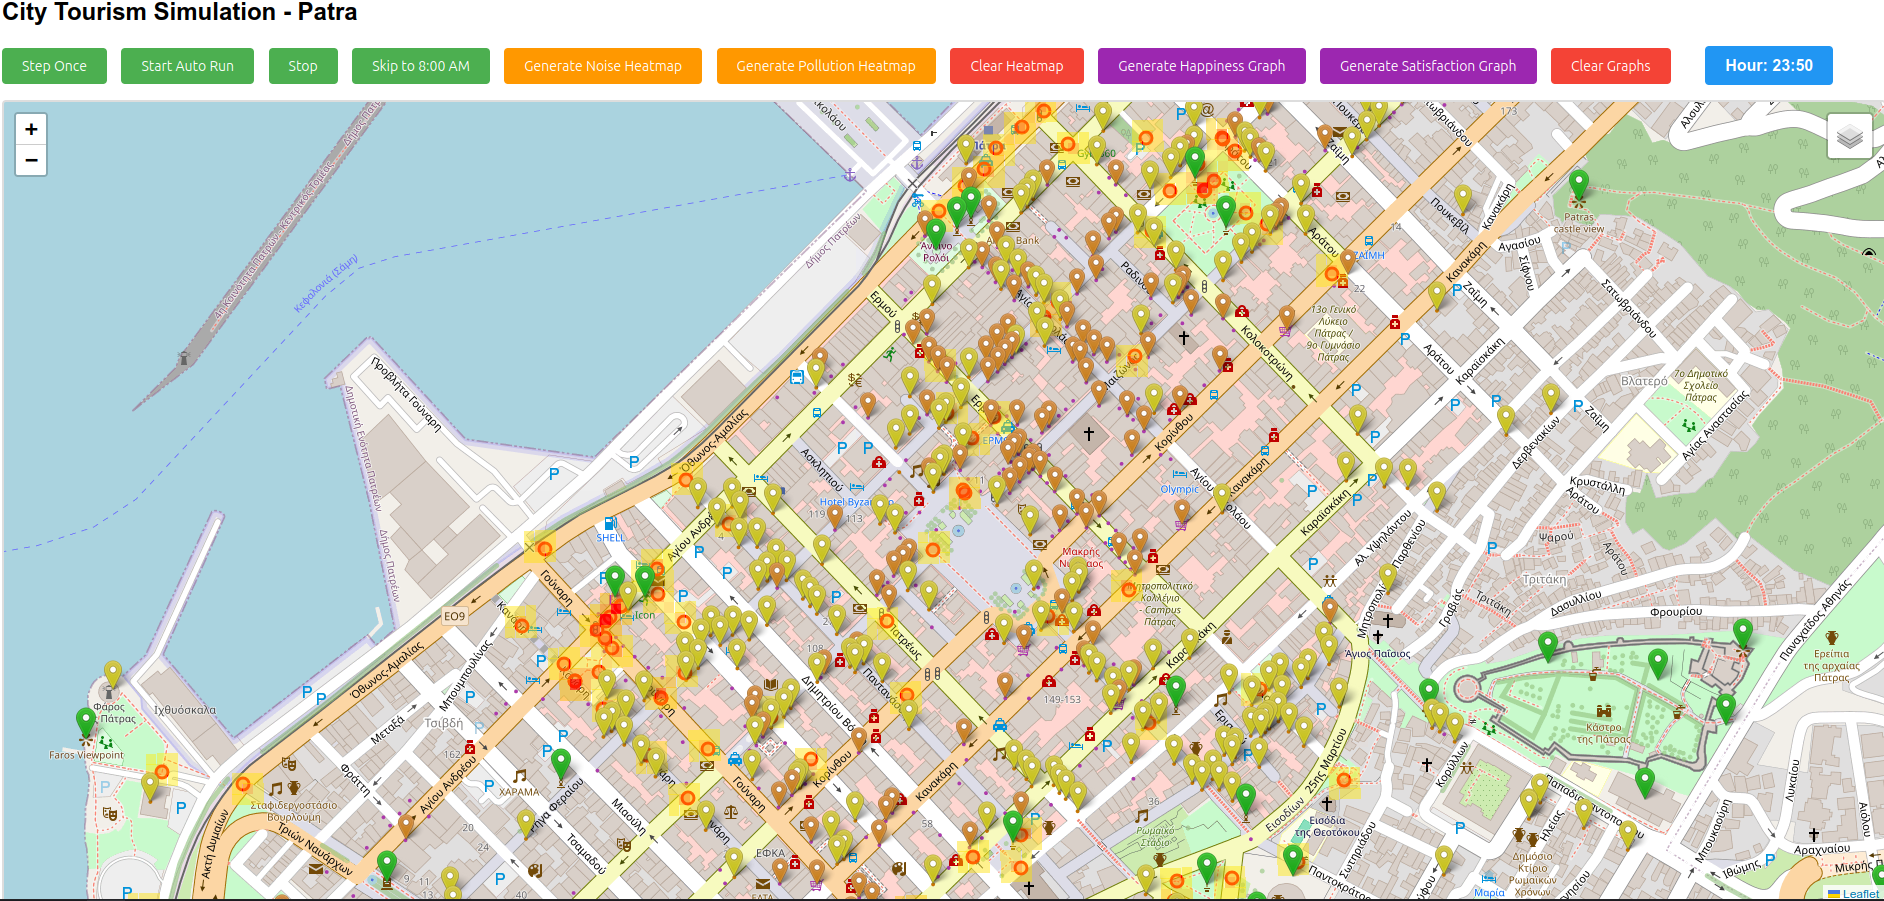
\includegraphics[width=\textwidth]{static/figures/noise_100_23.png}
\caption{100 τουρίστες (23:50)}\label{noise_100_23}
\end{figure}

\begin{figure}[H] \centering
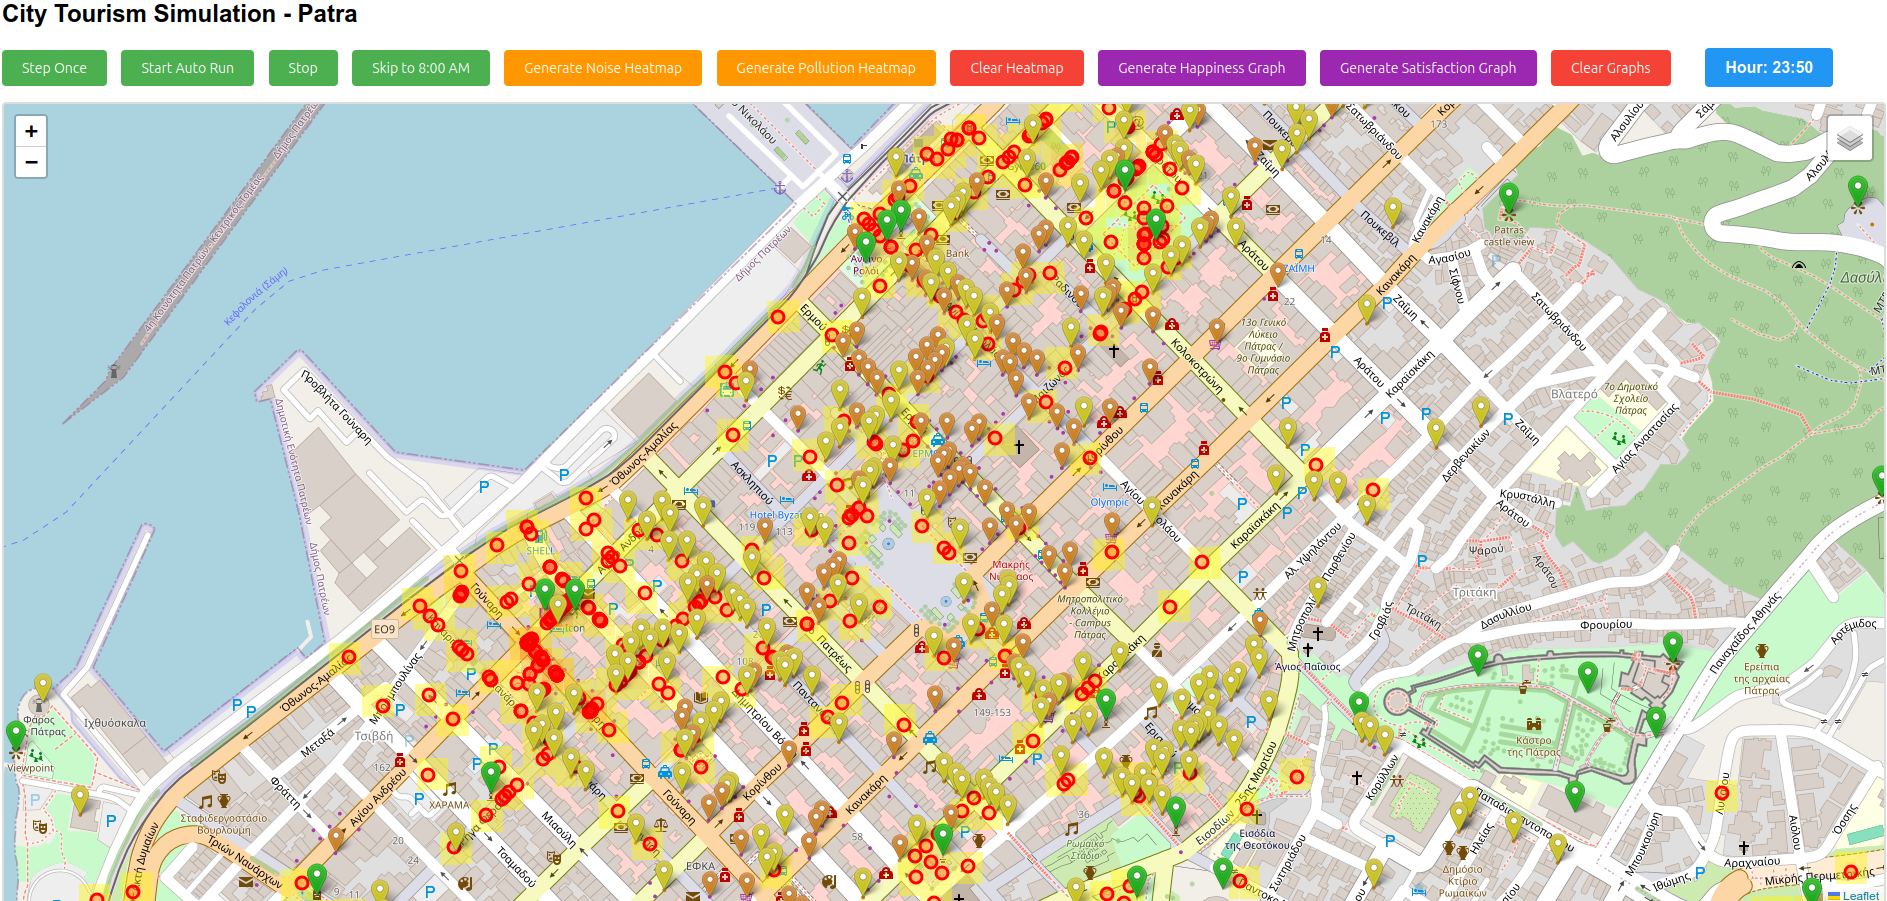
\includegraphics[width=\textwidth]{static/figures/noise_500_23.png}
\caption{500 τουρίστες (23:50)}\label{noise_500_23}
\end{figure}

\begin{figure}[H] \centering
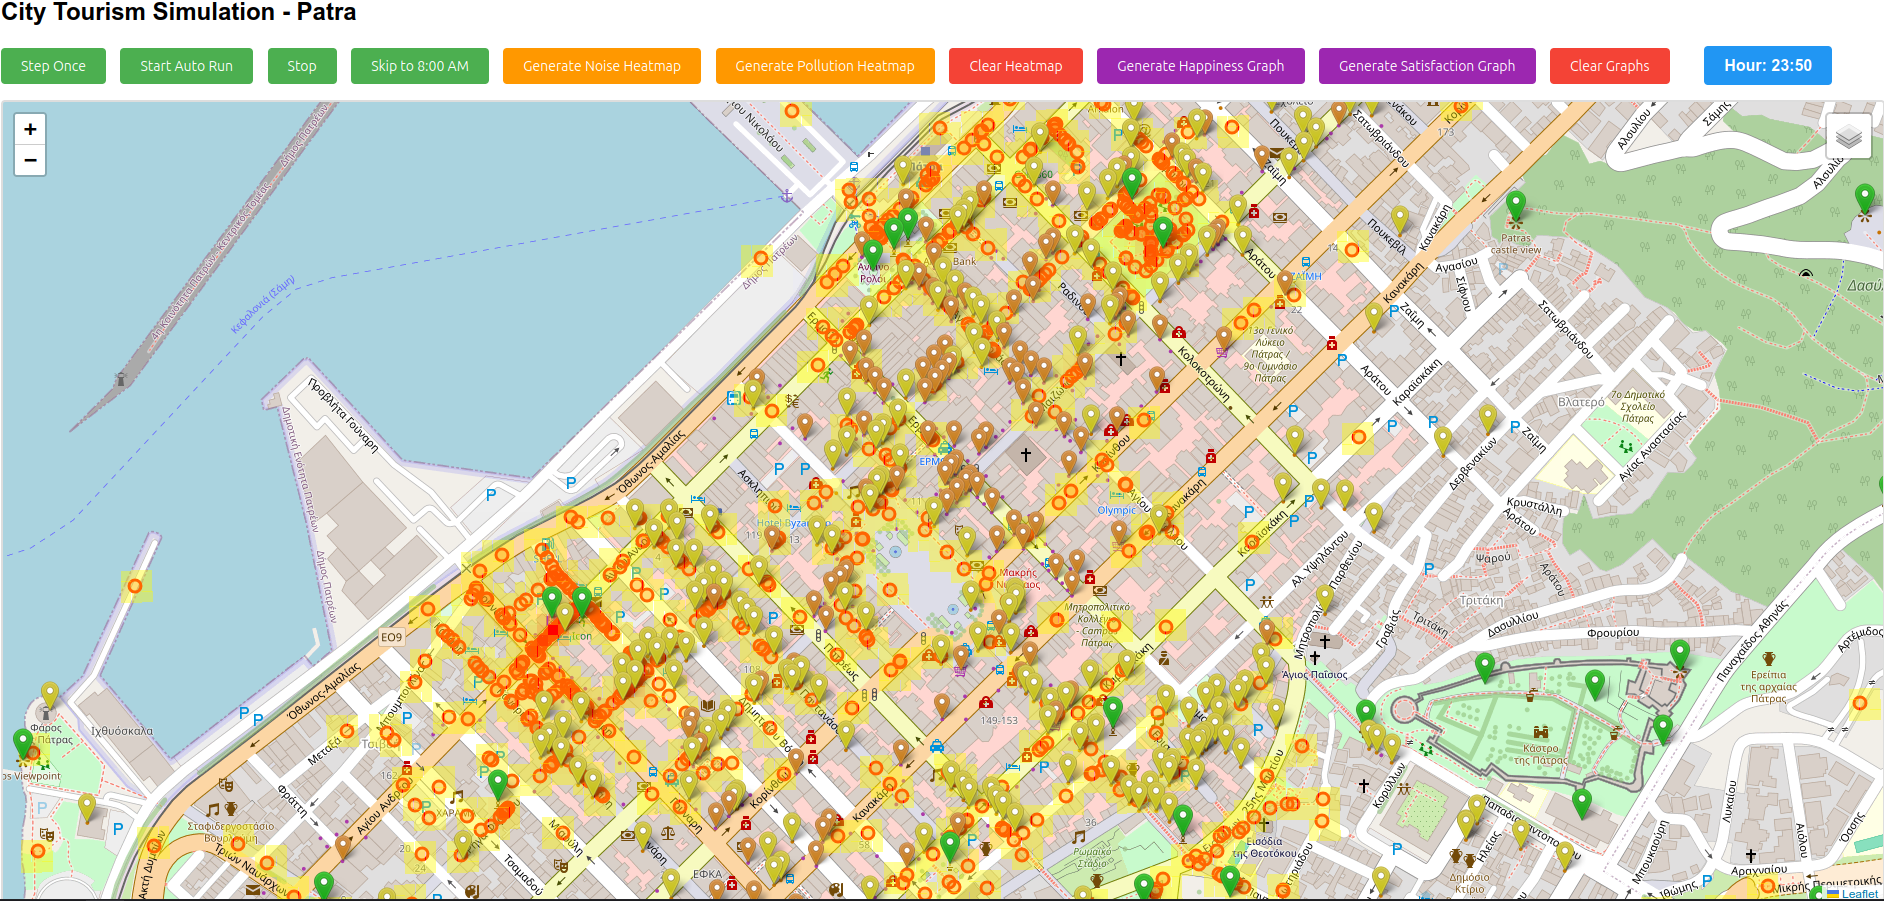
\includegraphics[width=\textwidth]{static/figures/noise_1000_23.png}
\caption{1000 τουρίστες (23:50)}\label{noise_1000_23}
\end{figure}

\section{Περιορισμοί Μοντέλου}

Παρά τα ενδιαφέροντα αποτελέσματα, το μοντέλο παρουσιάζει ορισμένους
περιορισμούς που πρέπει να ληφθούν υπόψη κατά την ερμηνεία των
αποτελεσμάτων.

Πρώτον, οι κάτοικοι είναι στατικοί πράκτορες. Στην πραγματικότητα,
οι κάτοικοι μιας πόλης κινούνται, αλλάζουν περιοχή και προσαρμόζουν
τη συμπεριφορά τους ανάλογα με τον τουρισμό. Η στατικότητά τους στο
παρόν μοντέλο σημαίνει ότι η επίδραση του τουρισμού στην ευτυχία τους
εξαρτάται αποκλειστικά από τυχαία αρχική τοποθέτηση, κάτι που εισάγει
σημαντικό στοιχείο τυχαιότητας στα αποτελέσματα.

Δεύτερον, τα χαρακτηριστικά θορύβου και ρύπανσης κάθε τουρίστα είναι
σταθερά τυχαίες τιμές στο [1, 2], χωρίς διαφοροποίηση βάσει τύπου οδού
ή βάσει κατάστασης (π.χ. διαφορετικές τιμές όταν ο τουρίστας είναι εν κινήσει
και διαφορετικές όταν είναι εντός \en{POI}). Επίσης, η διάχυση στα γειτονικά
κελιά του \en{heatmap} (30\% σταθερό ποσοστό) είναι απλοποιημένη σε σχέση με
ρεαλιστικά μοντέλα ακουστικής ή ατμοσφαιρικής ρύπανσης.

Τρίτον, η προσομοίωση εκτελείται μονονηματικά, γεγονός που περιορίζει την
κλιμάκωση σε μεγάλο αριθμό πρακτόρων. Παρότι ο κώδικας είναι ιδιαίτερα
αποδοτικός—καθώς το \en{Mesa} χρησιμοποιεί χωρική ευρετηρίαση
\en{(spatial indexing)} μέσω εσωτερικού πλέγματος \en{(internal grid)} για
την εύρεση γειτονικών πρακτόρων, ενώ για τον εντοπισμό κοντινών \en{POI}
αξιοποιήθηκε η δομή \en{KD-Tree}—η εκτέλεση περιορίζεται σε μερικές χιλιάδες
πράκτορες λόγω του συνολικού υπολογιστικού κόστους ανά χρονικό βήμα.

Τέλος, τα δεδομένα \en{OSM} για την Πάτρα δεν είναι πλήρη. Ορισμένα
ξενοδοχεία, \en{POI} ή τμήματα οδικού δικτύου ενδέχεται να απουσιάζουν
ή να είναι ανακριβή. Η ποιότητα των αποτελεσμάτων εξαρτάται άμεσα από
την πληρότητα των δεδομένων \en{OpenStreetMap} για την εκάστοτε πόλη.